\documentclass[letterpaper]{article}
\usepackage{aaai}
\usepackage{times}
\usepackage{helvet}
\usepackage{courier}
\usepackage{amsmath}
\usepackage{amssymb}
\usepackage{graphicx}
\usepackage{listings}
\usepackage{enumerate}
\frenchspacing
\setlength{\pdfpagewidth}{8.5in}
\setlength{\pdfpageheight}{11in}
\pdfinfo{l
/Title (Handwritten Font Generator Based on Pix2Pix)
/Author (Chengruidong Zhang, Haoran Xi)}
\setcounter{secnumdepth}{0}  
 \begin{document}
% The file aaai.sty is the style file for AAAI Press 
% proceedings, working notes, and technical reports.
%
\title{Handwritten Font Generator Based on Pix2Pix}
\author{Chengruidong Zhang, Haoran Xi}
\maketitle

\section{Problem Statement}
A font consists of a set of character images sharing the same style. Because each character has a fixed skeleton, we may be able to extract the style information from limited character images and apply it to all characters. This means that a new font can be created with very few character images as input, and everyone can create his / her handwritten font without writing all the characters.

\begin{center}
    
\includegraphics[]{update-fig-sample.png}

    Figure 1. Same characters in different fonts.
\end{center}


\section{Related Works}
\subsection{Image Style Transfer Using CNN}
It is an algorithm that can separate and recombine the image content and style of natural images. A Convolutional Neural Network is trained to extract high level image information and produce new images of high perceptual quality that combine the content of an arbitrary photograph with the appearance of specified artworks.
\\
This work proves the feasibility of using CNN for image style transfer and creatively introduced the style transfer loss, which feeds the predicted and target images into a pre-trained CNN and compares every hidden layers to judge the consistency in texture.

\subsection{StyleGAN}
StyleGAN is a GAN architecture with a style-based generator that receives additional inputs to adjust the style. It leads to an automatically learned, unsupervised separation of high-level attributes and stochastic variation in the generated images, and it enables intuitive, scale-specific control of the synthesis.
\\
Unlike the traditional CNN decoder, StyleGAN adds an adaptive instance normalization (AdaIN) function to each convolution layer, where additional information is introduced to adjust the style.
\\
StyleGAN has an inspiring feature as known as Style Mixing, which allows the generator to mix the basic features (skeleton) of one image with the advanced features (style) of another image by applying their latent codes at different levels.

\subsection{Pix2pix}
Pix2pix is a conditional GAN which trains a generator that translate images to images. This is an end-to-end approach that is more straight than StyleGAN.
\\
The generator model is usually constructed as a U-Net, which contains symmetrical downscaling and upscaling convolution blocks and cross-layer connections between modules of the same resolution.
\\
Pix2pix can also be used to produce a group of pixel-wise correlated input images concatenated in channels, such as a line draft and corresponding colors, a photo and its labels, etc. 

\subsection{Wasserstein GAN}
The Wasserstein Generative Adversarial Network is an extension to the generative adversarial network that both improves the stability when training the model and provides a loss function that correlates with the quality of generated images.
\\
Using Wasserstein loss, we can effectively avoid the training of the generator falling behind or ahead of the discriminator given the same training frequency.


\section{Dataset}
The dataset includes $32 \times 32$ single-channel (black and white) images of common characters extracted from 14 different hand-written font files provided by Google Fonts: Bradley Hand ITC, Caveat, Comic Sans MS, Cookie, Fuzzy Bubbles, Gloria Hallelujah, Indie Flower, Ink free, Mali, Ole, Sacramento, Shadows into Light, Twinkle Star and Vujaday Script.
\begin{center}
    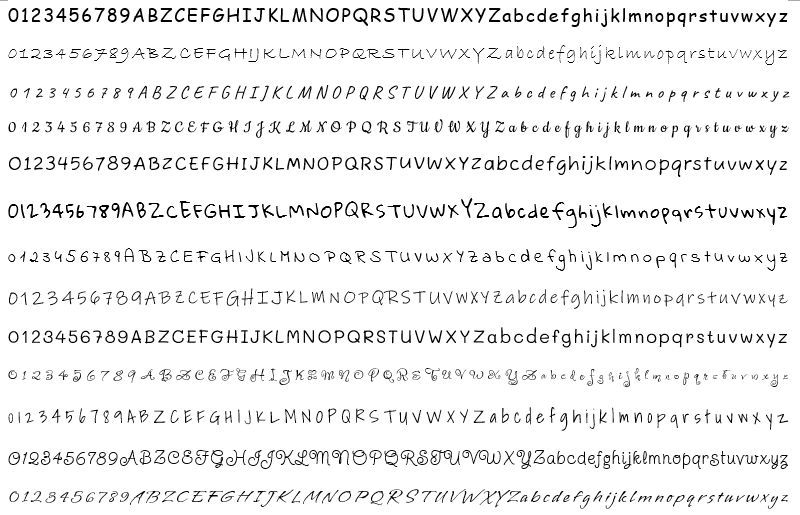
\includegraphics[width=8cm]{report-fig-dataset.png}

    Figure 2. The whole dataset consisting of 14 fonts.\\The first line is extracted from the Comic font,\\ which is the base font described in the next section.
\end{center}
The dataset is generated by a render module which can extract images of specific characters from True Type font files. Except the base font Comic, 9 in 13 fonts are configured as training fonts, 2 validation fonts and 2 test fonts. 80\% characters in training fonts are randomly picked for training and the remaining 20\% are used for validation and test along with validation and test fonts.

\section{Model}
We built a Generative Adversarial Network, which consists of a discriminator and a generator. The discriminator predicts $D(x,y)=P(y|x)$, which means the probability that the output image $y$ is true given input images $x$. The generator generates the predicted output image $\hat{y}=G(x)$ and makes the output judged as true by the discriminator as much as possible.
\\
The discriminator is designed as a 5-layer CNN classifier with 1 output class. The generator can be either a StyleGAN generator or a U-Net generator.
\\
Denote an image of character $i$ and font $F_k$ by $F_k[i]$. For each training iteration, the generator takes a pair of images $(x_1=F_0[i], x_2=F_k[j])$ and outputs an image $\hat{y}=G(x)$ with skeleton of $x_1$ and style of $x_2$. The discriminator judges both $P(y|x)=D(x,y)$ and $P(\hat{y}=D(x,\hat{y}))$, where the groundtruth image $y=F_k[i]$. Font $F_0$ is the base font, which should have clear skeletons, and can be the same whenever training or testing.

\subsection{StyleGAN Generator}
This is the generator model what we first envisaged, which is modified from the basic StyleGAN generator. The original full-connected mapping network is replaced by an convolutional network to extract style information directly from input images.

\begin{center}
    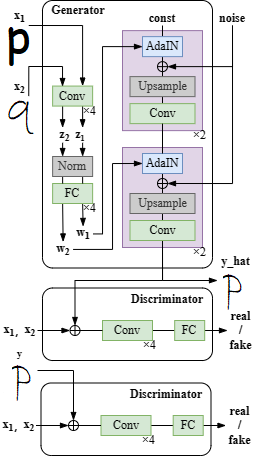
\includegraphics[]{report-fig-model-1.png}

    Figure 3. Structure of our end-to-end StyleGAN\\generator and discriminator. The generator includes\\a Mapping Network and a Synthesis Network. The\\Mapping Network consists of a 4-layer CNN encoder\\and a 4-layer full-connected network. The Synthesis\\Network is a 4-layer CNN decoder with AdaIN.
\end{center}
On each training epoch, two images of different fonts are fed into the downscaling network on the left to produce intermediate vectors $w_1$ and $w_2$. In the upsacling network on the right, the one providing the skeleton will be used for the lower part of the decoder, and the one providing the style will be used for the upper part.

\subsection{U-Net Generator}
Since the end-to-end StyleGAN generator did not meet our expectations after preliminary training, we tried pix2pix U-Net generator instead.
\\
It is a traditional pix2pix U-Net Generator with 4 downscaling blocks and 4 upscaling blocks. The inputs and outputs are the same with previous end-to-end StyleGAN Generator, where $x_1$ and $x_2$ are concatenated in the channel dimention and input to the first downscaling block as a whole $32 \times 32 \times 2$ image.
\\
\begin{center}
    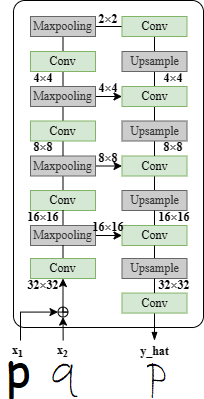
\includegraphics[]{report-fig-model-2.png}

    Figure 4. Structure of our pix2pix generator.
\end{center}

\section{Training}
We followed the basic GAN training process:
\begin{lstlisting}
For each epoch
    For each iteration
        Get next training data (x1, x2, y)
        Forward Generator:
            y_pred = F(x1, x2)
        Forward Discriminator:
            pred_fake = D(y_pred, x1, x2)
            pred_real = D(y, x1, x2)
        Freeze gradients of Generator
        Backward and optimize Discriminator
        Freeze gradients of Discriminator
        Backward and optimize Generator
    Run evaluation
Run test
\end{lstlisting}
We choose Adam optimizer to optimize parameters. The optimization goal is:
$$\begin{aligned}
\min_{D} V_{GAN}(D)\\
\min_{G} V_{GAN}(G)
\end{aligned}$$
The loss function $V$ can be either least squares or Wasserstein loss.
\\
For least squares loss,
$$\begin{aligned}
    V_{GAN}(D) &= \frac12E[D^2(G(x))]+\frac12E[(1-D(y))^2]\\
    V_{GAN}(G) &= \frac12E[(1-D(G(x)))^2]
\end{aligned}$$
For Wasserstein loss,
$$\begin{aligned}
    V_{GAN}(D) &= \frac12\left(E[D(G(x))]-E[D(y)]\right)\\
    V_{GAN}(G) &= -\frac12E[D(G(x))]
\end{aligned}$$
Note that the training process of generator and discriminator can be unbalanced when we choose the least squares loss. We can adjust the ratio of training frequency of $G$ and $D$ to rebalance them.
\\
For U-Net generator, we can also add a $l1$-loss term to the generator's loss function to make the model converge in the early stage:
$$V_{L1}(G) = |y-G(x)|$$

\subsection{Hyperparameter Selection}
Here are the adjustable hyperparameters during training process:
\begin{table}[h]
    \centering
    \begin{tabular}{|l|c|}
        \hline
        Hyperparameter&Default Value\\
        \hline
        Epoch Number&100\\
        Iteration Number&2000\\
        Batch Size&8\\
        Optimizer&Adam\\
        Learning Rate&0.01\\
        GAN loss&Least Squares\\
        G/D Training Ratio&10\\
        \hline
    \end{tabular}
    \caption{Hyperparameters for GAN}
\end{table}

\begin{table}[h]
    \centering
    \begin{tabular}{|l|c|}
        \hline
        Hyperparameter&Default Value\\
        \hline
        Mapping Network Layers&4\\
        Synthesis Network Layers&4\\
        Interval Vector Size&512\\
        Add Noise&None\\
        \hline
    \end{tabular}
    \caption{Hyperparameters for StyleGAN Generator}
\end{table}

\begin{table}[h]
    \centering
    \begin{tabular}{|l|c|}
        \hline
        Hyperparameter&Default Value\\
        \hline
        Downscaling Layers&4\\
        Upscaling Layers&4\\
        L1 loss weight&10\\
        \hline
    \end{tabular}
    \caption{Hyperparameters for U-Net Generator}
\end{table}

Because we didn't get an acceptable result on the StyleGAN generator, we will mainly discuss hyperparameter tunning on the U-Net generator is this section.
\\
To quantify the quality of the generated image $\hat{y}$, we print out the negative cosine simularity and the minimum squared error between $y$ and $\hat{y}$ on the evaluation dataset after each epoch. Note that these two measures should be roughly equal for 1-channel images.

\subsection{Whether to Use L1 Loss}
First, we run two experiments with and without $l1$-loss, respectively.
\begin{center}
    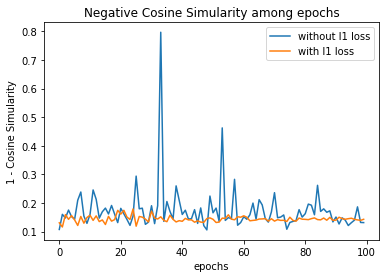
\includegraphics[width=.5\textwidth]{./report-fig-hp-1.png}

    Figure 5. Negative cosine simularity among epochs with and without $l1$-loss
\end{center}
It can be seen from the figure that L1 loss function can effectively prevent the training process from developing to an unstable direction.

\subsection{Basic Hyperparameter Selection}
We decided to change 1 hyperparameter a time which are 6 models totally. The measurement of these models are the mse loss of $y$ and $\hat{y}$ we generate. We compute the loss every epoch for validation dataset. Here is a figure of the loss per sample among epochs.

\begin{center}
    \includegraphics[width=.5\textwidth]{./update-figs/MSE loss among epochs.png}

    Figure 6. MSE Loss among epochs for 6 different models.
\end{center}

From this figure, we found that using lsgan loss funtion could make the model perform better. And for only lsgan models, we have plot them in a separate figure shown below. In this figure, we observed when learning rate is enlarge to 0.03, the model performs better, and when $gdrate$ is reduced to 1, the model perform worst. Since the default setting is the second best, we believe the hyperparameters $lr=0.03$, $batchsize=8$, $gdrate=10$ and $GAN loss=lsgan$ is a fairly good parameter setting.

\begin{center}
    \includegraphics[width=.5\textwidth]{./update-figs/MSE loss among epochs without wgan.png}

    Figure 7. MSE Loss among epochs without wgan for 5 different models.
\end{center}

\subsection{Advanced Hyperparameter Selection}
Then we optimized the unet architecture in 3 ways. First, we add another convolution layer to the end to optimize the output quality; secondly, we change the ReLU layers in the U-Net into leaky ReLU layers to avoid the "dead ReLU" problem and make the model more robust; thirdly, we tried use the nearest mode in upsample layers.
\\
We also trained original unet model for another 100 epochs, which is 200 epochs in total.

\begin{center}
    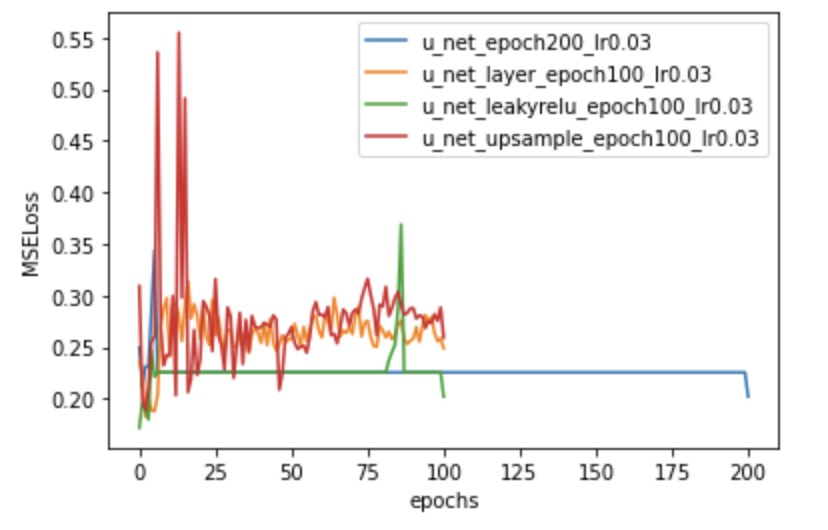
\includegraphics[width=.5\textwidth]{./report-fig-hp-2.jpeg}

    Figure 8. MSEloss results of Updating\\U-Net in 4 different ways.
\end{center}

From the images above, we can discover that the MSEloss of 200 epochs model has not changed after epoch 25, so it has converged for 100 epoch models. And the U-Net with leaky ReLU layer performs better than the others, it shows that the leaky ReLU is more suitable for the GAN training process.
\\
The U-Net with an additional convolution layer and the one with nearest mode upsample layers, performs quite similar and have larger MSEloss. Therefore, these two optimizations are not effective enough.

\section{Results}
\subsection{StyleGAN Generator}
As we mentioned before, our end-to-end StyleGAN Generator does not converges during the training process.

\begin{center}
    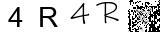
\includegraphics[width=.2\textwidth]{./update-figs/e2estylegan_1.jpg}
    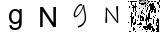
\includegraphics[width=.2\textwidth]{./update-figs/e2estylegan_2.jpg}\\
    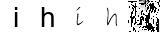
\includegraphics[width=.2\textwidth]{./update-figs/e2estylegan_3.jpg}
    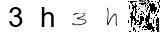
\includegraphics[width=.2\textwidth]{./update-figs/e2estylegan_4.jpg}\\
    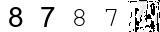
\includegraphics[width=.2\textwidth]{./update-figs/e2estylegan_5.jpg}
    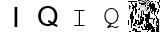
\includegraphics[width=.2\textwidth]{./update-figs/e2estylegan_6.jpg}\\

    Figure 9. A typical test output of our\\StyleGAN generator. From left to right:\\$x_0=F_0[i]$ (not as input), $x_1=F_0[j]$,\\$x_2=F_k[i]$, $y=F_k[j]$, $\hat{y}=G(x_1,x_2)$
\end{center}

\subsection{U-Net Generator}
\subsubsection{Test Outputs}
Train a U-Net generator under the best hyperparameters described in the previous sector, we get some sampled test outputs:

\begin{center}
    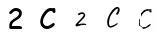
\includegraphics[width=.2\textwidth]{./report-figs/1.caveat.1.jpg}
    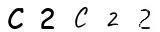
\includegraphics[width=.2\textwidth]{./report-figs/1.caveat.2.jpg}\\
    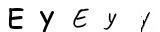
\includegraphics[width=.2\textwidth]{./report-figs/1.caveat.3.jpg}
    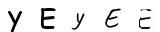
\includegraphics[width=.2\textwidth]{./report-figs/1.caveat.4.jpg}\\
    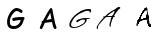
\includegraphics[width=.2\textwidth]{./report-figs/1.vujah.1.jpg}
    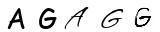
\includegraphics[width=.2\textwidth]{./report-figs/1.vujah.2.jpg}\\
    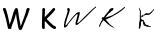
\includegraphics[width=.2\textwidth]{./report-figs/1.vujah.3.jpg}
    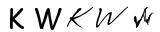
\includegraphics[width=.2\textwidth]{./report-figs/1.vujah.4.jpg}\\

    Figure 10. sampled pairs in U-Net test results for the two test fonts. The target fonts of the 2 top rows and the 2 bottom rows are Caveat and Vujaday Script, respectively.
\end{center}

\begin{center}
    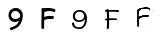
\includegraphics[width=.2\textwidth]{./report-figs/2.mali.1.jpg}
    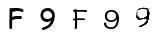
\includegraphics[width=.2\textwidth]{./report-figs/2.mali.2.jpg}\\
    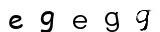
\includegraphics[width=.2\textwidth]{./report-figs/2.mali.3.jpg}
    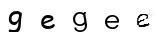
\includegraphics[width=.2\textwidth]{./report-figs/2.mali.4.jpg}\\
    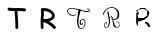
\includegraphics[width=.2\textwidth]{./report-figs/2.ole.1.jpg}
    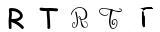
\includegraphics[width=.2\textwidth]{./report-figs/2.ole.2.jpg}\\
    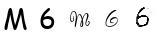
\includegraphics[width=.2\textwidth]{./report-figs/2.ole.3.jpg}
    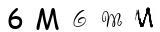
\includegraphics[width=.2\textwidth]{./report-figs/2.ole.4.jpg}\\

    Figure 11. sampled pairs in U-Net test results for\\several test characters of two training fonts.\\The target fonts of the 2 top rows and the\\2 bottom rows are Mali and Ole, respectively.
\end{center}

The above results show that the trained U-Net generator has the basical ability to parse style information from one character picture and add it to another character picture. It can sense and apply the thickness change and curvature of strokes.
\\
However, it performs not good on the Ole font. It's still hard to learn to add decorations to characters, such as redundant corners and circles. It may be limited by the structure of U-Net and our loss functions.

\subsubsection{Validation Outputs}
Next, let's look at several validation outputs in the training process:

\begin{center}
    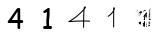
\includegraphics[width=.2\textwidth]{./report-figs/3.sac.1.jpg}
    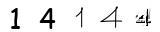
\includegraphics[width=.2\textwidth]{./report-figs/3.sac.2.jpg}\\
    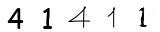
\includegraphics[width=.2\textwidth]{./report-figs/3.sac.3.jpg}
    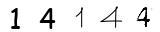
\includegraphics[width=.2\textwidth]{./report-figs/3.sac.4.jpg}\\
    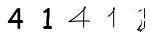
\includegraphics[width=.2\textwidth]{./report-figs/3.sac.5.jpg}
    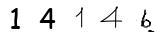
\includegraphics[width=.2\textwidth]{./report-figs/3.sac.6.jpg}\\
    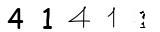
\includegraphics[width=.2\textwidth]{./report-figs/3.sac.7.jpg}
    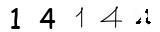
\includegraphics[width=.2\textwidth]{./report-figs/3.sac.8.jpg}\\

    Figure 12. sampled pairs in U-Net validation results for the validation font Sacramento. Each row is taken from the 10th, 30th, 60th and 99th epochs respectively.
\end{center}
The validation outputs shows that the training process converges faster than we expected, but not stable after that. The results of the 60th epoch and the 99th epoch are not as good as the results of the 30th epoch. It may because our learning rate is too high, and the discriminator is too simple to judge the reality on all 14 fonts and 36 characters.

\subsubsection{Comparison between Generator Loss and Discriminator Loss}
We printed the average GAN loss of generaor ($l1$-loss not included) and discriminator during the 100 epochs:

\begin{center}
    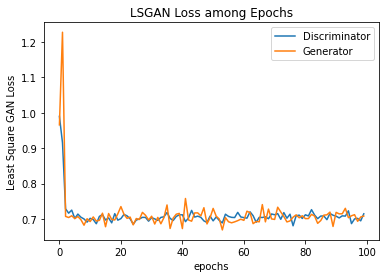
\includegraphics[width=.5\textwidth]{./report-fig-gd.png}

    Figure 13. LSGAN Loss in the training process.
\end{center}
According to the figure, the GAN losses of generator and discriminator are relatively stable at about 0.7. We think this is a healthy proportion for our generator and discriminator to progress together.

\section{Conclusion}
\begin{itemize}
    \item We designed and built two GAN models to train a end-to-end CNN generator with the ability of transfering font styles.
    \item Through experiments, we confirmed that the modified StyleGAN generator is not suitable for this end-to-end task.
    \item We have made a simple adjustment and improvement to U-Net, so that it has the basical ability of font style transfering.
    \item The U-Net still cannot handle complex fonts with redundant decorations.
\end{itemize}

\section{Reference}
\smallskip \noindent
Leon, A. G., Alexander, S. E., and Matthias, B. 2016. Image Style Transfer Using Convolutional Neural Networks. \textit{CVPR}, pp. 2414-2423.

\smallskip \noindent
Tero, K., Samuli, L., and Timo, A. 2019. A Style-Based Generator Architecture for Generative Adversarial Networks. \textit{CVPR}, abs/1812.04948.

\smallskip \noindent
Ko, D. H., Hassan, A. U., Suk, J., \& Choi, J. 2021. SKFont: skeleton-driven Korean font generator with conditional deep adversarial networks. \textit{International Journal on Document Analysis and Recognition (IJDAR)}, 1-13.

\smallskip \noindent
Bhunia, A. K., Bhunia, A. K., Banerjee, P., Konwer, A., Bhowmick, A., Roy, P. P., \& Pal, U. 2018. Word level font-to-font image translation using convolutional recurrent generative adversarial networks. \textit{ICPR} (pp. 3645-3650).


\section{Appendix}
Our code repository: https://github.com/Starmys/FontStyleTransfer

\bibliography{proposal-reference.bib}
\bibliographystyle{aaai}
\end{document}